\documentclass{article}
\usepackage{amsmath,amsthm,amssymb}
\usepackage {mathtext}
\usepackage{amsfonts} 
\usepackage[T1,T2A]{fontenc}
\usepackage[utf8]{inputenc}
\usepackage [english, russian] {babel}
\usepackage[babel=true]{microtype}
\usepackage{caption}
\usepackage{subcaption}
\captionsetup[table]{position=t,justification=raggedleft,slc=off}
\setlength{\abovecaptionskip}{0pt}
\usepackage {geometry}
\usepackage{graphicx}
\usepackage{multirow}
\usepackage{booktabs}
\usepackage{pgfplots}
\pgfplotsset{compat=1.18}
\geometry{margin=2cm}
\title{Отчёт о лабораторной работе №2.4.1. \\ Определение теплоты испарения жидкости}
\author{Павел Рудачихин, группа Б04-507}
\date{12.02.2026}
\begin {document}
\maketitle

	
\section*{Аннотация}
	
	\hspace{4mm} \textbf{Цель работы:} измерить давления насыщенного пара жидкости (воды) в зависимости от температуры и вычислить молярную теплоту испарения с помощью уравнения Клапейрона–Клаузиуса.
	
	\textbf{Оборудование:} термостат, запаянный стеклянный прибор с исследуемой жидкостью, U-образный ртутный манометр, отсчётный микроскоп.
	
	\textbf{Метод:} Косвенный метод, основанный на измерении производной \(dP/dT\) кривой насыщения. Экспериментально получается зависимость \(P(T)\) путём измерения давления пара при различных температурах термостата. Затем, используя упрощённое уравнение Клапейрона–Клаузиуса, рассчитывается молярная теплота испарения.
	
\section*{Теоретические сведения}
	
	\hspace{4mm} Испарение — это фазовый переход первого рода. Согласно уравнению Клапейрона–Клаузиуса, наклон кривой фазового равновесия жидкость–пар определяется выражением:
	\begin{equation}
		\frac{dP}{dT} = \frac{L}{T(V_2 - V_1)},
	\end{equation}
	где \(P\) — давление насыщенного пара, \(T\) — абсолютная температура, \(L\) — молярная теплота испарения, \(V_2\) и \(V_1\) — молярные объёмы пара и жидкости соответственно.
	
	При давлениях ниже атмосферного (вдали от критической точки) можно пренебречь объёмом жидкости (\(V_2 \gg V_1\)), а пар считать идеальным газом (\(V_2 = RT/P\)). Подстановка этих допущений в уравнение (1) даёт расчётную формулу:
	\begin{equation}
		L = \frac{RT^2}{P} \frac{dP}{dT} = -R \frac{d(\ln P)}{d(1/T)} \label{eq:final}
	\end{equation}
	Таким образом, для нахождения \(L\) необходимо экспериментально определить зависимость \(P(T)\), построить график в координатах \(\ln P\) от \(1/T\) и найти его угловой коэффициент.
	
\section*{Экспериментальная установка}
	
	\begin{figure}[h!]
		\centering
		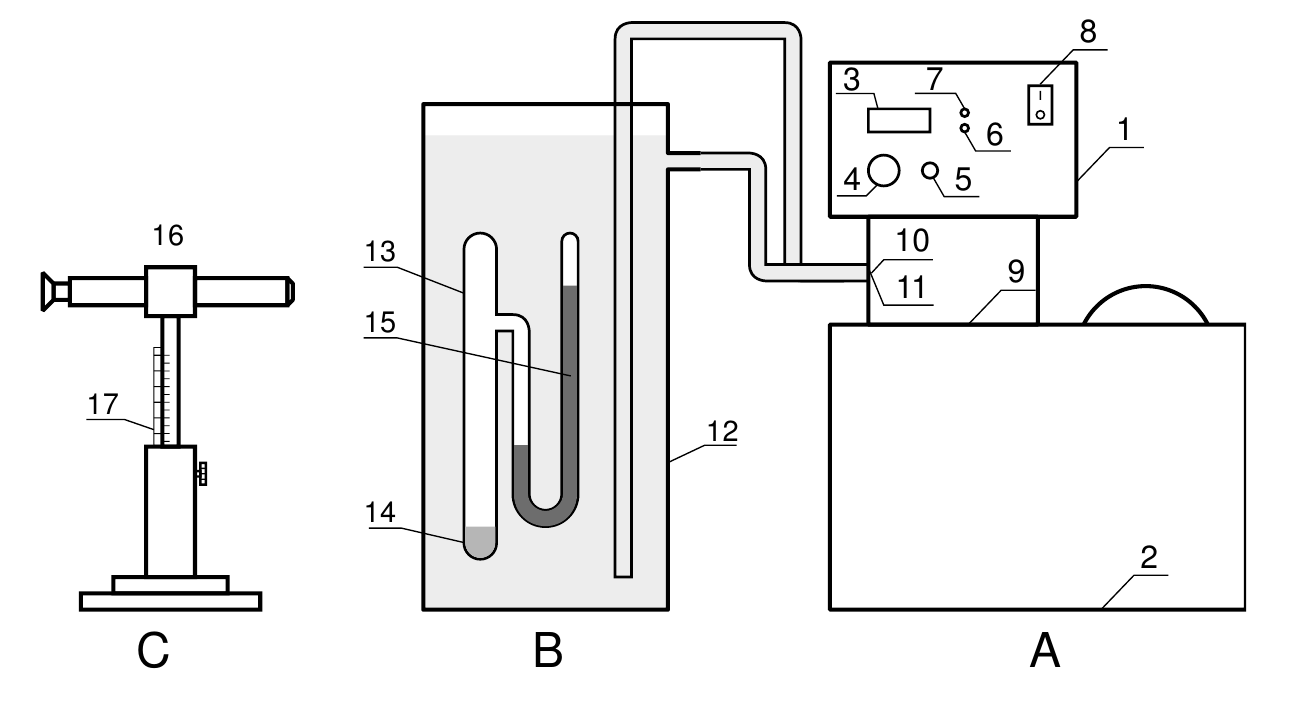
\includegraphics[width=0.6\textwidth]{1.png}
		\caption{Схема установки: А - емкость термостата (в реальности не обособлена), В - рабочая ёмкость, С - стойка отсчётного микроскопа (в реальности закреплена на корпусе В), 1-11 - термостат и его элементы, 12 - ёмкость с водой, 13 - запаянный прибор, 14 - исследуемая жидкость, 15 - ртутный манометр, 16 - отсчётный микроскоп, 17 - шкала микроскопа.}
		\label{fig:setup2}
	\end{figure}
	
	\hspace{4mm} Используемая в работе установка (рис. 1) включает в себя циркуляционный термостат (А) с точной регулировкой температуры. Экспериментальный прибор (В) представляет собой ёмкость (12) с водой, в которую погружен запаянный сосуд (13) с исследуемой жидкостью (14). Давление пара измеряется ртутным манометром (15). Отсчёт положения менисков ртути производится с помощью микроскопа (16), перемещающегося по вертикальной шкале (17).
	
	
	
\section*{Результаты измерений}

	\hspace{4mm} В ходе эксперимента была измерена разность уровней ртути в U-образном манометре \( \Delta h \) при различных температурах \( t \) (в °C). Измерения проводились как при нагревании, так и при охлаждении системы для контроля стабильности и отсутствия гистерезиса. Давление насыщенного пара \(P\) измерено непосредственно микроскопом в мм.рт.ст.
	
	Полученные данные сведены в Таблицу 1. Для дальнейшей обработки температура переведена в Кельвины (\(T = t + 273,15\)).
	
	\begin{table}[h!]
		\centering
		\captionbox{Экспериментальные данные давления насыщенного пара воды}{		\label{tab:data}
		\begin{tabular}{|c|c|c||c|c|c|}
			\hline
			\multicolumn{3}{|c||}{Нагревание} & \multicolumn{3}{|c|}{Охлаждение} \\
			\hline
			\(t\), °C & \(P\), мм рт. ст. & \(T\), К & \(t\), °C & \(P\), мм рт. ст. & \(T\), К \\
			\hline
			22,0 & 27,62 & 295,15 & 39,0 & 73,33 & 312,15 \\
			23,1 & 29,73 & 296,25 & 38,0 & 68,62 & 311,15 \\
			24,1 & 30,89 & 297,25 & 37,0 & 65,53 & 310,15 \\
			25,1 & 33,45 & 298,25 & 36,0 & 63,19 & 309,15 \\
			26,1 & 34,26 & 299,25 & 35,0 & 58,87 & 308,15 \\
			27,1 & 37,08 & 300,25 & 34,0 & 56,52 & 307,15 \\
			28,1 & 39,09 & 301,25 & 33,0 & 53,71 & 306,15 \\
			29,1 & 41,18 & 302,25 & 32,0 & 50,49 & 305,15 \\
			30,1 & 44,29 & 303,25 & 31,0 & 48,80 & 304,15 \\
			31,0 & 46,67 & 304,15 & 30,0 & 45,80 & 303,15 \\
			32,0 & 49,53 & 305,15 & 29,0 & 43,57 & 302,15 \\
			33,0 & 51,76 & 306,15 & 28,0 & 41,12 & 301,25 \\
			34,0 & 54,83 & 307,15 & 27,0 & 38,25 & 300,25 \\
			35,0 & 57,96 & 308,15 & 26,0 & 36,13 & 299,25 \\
			36,0 & 61,01 & 309,15 & & & \\
			37,0 & 64,33 & 310,15 & & & \\
			38,0 & 67,80 & 311,15 & & & \\
			39,0 & 71,36 & 312,15 & & & \\
			40,0 & 75,41 & 313,15 & & & \\
			\hline
			\end{tabular}}
	\end{table}
	
\section*{Обработка результатов}

	\hspace{4mm} Обработка экспериментальных данных проводилась методом наименьших квадратов (МНК) для нахождения производной \(d(\ln P)/d(1/T)\).
	
	1.  \textbf{Построение графика \(P(T)\).} На графике (Рис. 3) были нанесены экспериментальные точки для режимов нагревания и охлаждения. Наблюдается хорошая сходимость точек, что подтверждает отсутствие значительного перегрева или переохлаждения жидкости относительно температуры термостата. Кривая имеет экспоненциальный характер, что соответствует физическому смыслу (уравнению Клапейрона–Клаузиуса).
	
	\begin{figure}[h!]
		\centering
		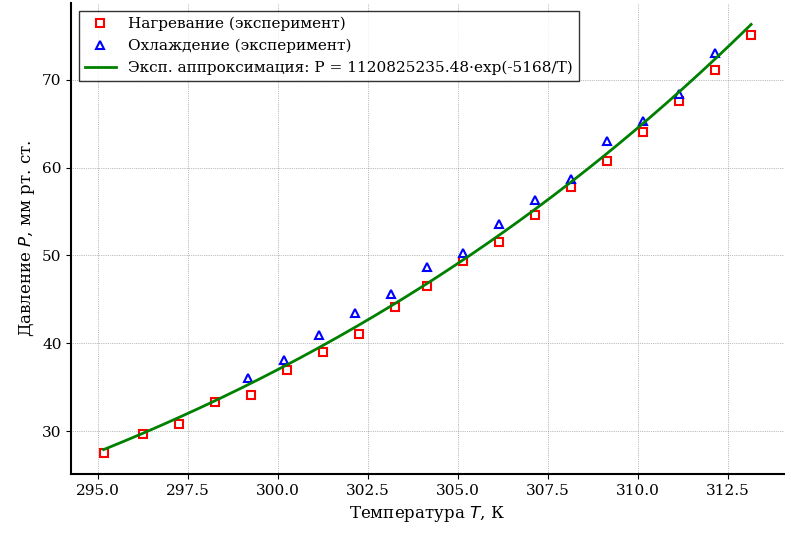
\includegraphics[width=0.8\textwidth]{F1.png}
		\caption{График зависимости P(T)}
		\label{fig:P_T}
	\end{figure}
	
	2.  \textbf{Линеаризация графика.} Для определения углового коэффициента был построен график в линеаризованных координатах \(\ln P\) от \(10^3/T\) (Рис. 4). Использование множителя \(10^3\) удобно для представления чисел на графике. Все экспериментальные точки (для нагрева и охлаждения) с хорошей точностью аппроксимируются единой прямой линией. Это подтверждает возможность использования упрощённой формулы \eqref{eq:final} и линейный характер зависимости \(\ln P\) от \(1/T\).
	
	\begin{figure}[h!]
		\centering
		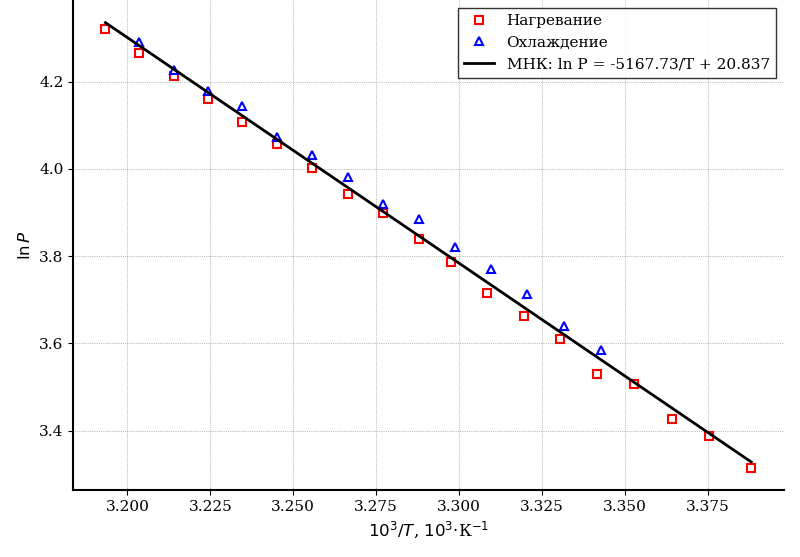
\includegraphics[width=0.8\textwidth]{F2.png}
		\caption{График зависимости $\ln P(1/T)$}
		\label{fig:lnP_1_T}
	\end{figure}
	
	Угловой коэффициент прямой, определённый методом наименьших квадратов, составляет:
	\[
	\frac{d(\ln P)}{d(1/T)} = -5250 \ К 
	\]
	
	\section*{Оценка погрешностей}
	
	1.  \textbf{Погрешность измерения температуры \(\Delta T\).} Температура измерялась лабораторным термометром с ценой деления 0,1 °C. С учётом возможной разницы температур между термостатом и исследуемой жидкостью, абсолютная погрешность принята равной \(\Delta T = \pm 0.2\) К.
	
	2.  \textbf{Погрешность измерения давления \(\Delta P\).} Давление определялось по разности высот столба ртути с помощью микроскопа. Цена деления отсчётной шкалы микроскопа составляет 0,01 мм. Следовательно, инструментальная погрешность измерения давления \(\Delta P = \pm 0,01\) мм рт. ст. Относительная погрешность \(\varepsilon_P = \Delta P / P\) максимальна при минимальных давлениях и составляет менее 0,04\%.
	
	3.  \textbf{Погрешность определения углового коэффициента.} Основной вклад в погрешность конечного результата вносит погрешность определения углового коэффициента наклона прямой на графике \(\ln P\) от \(1/T\). Согласно методу наименьших квадратов, стандартная ошибка наклона составляет \(\sigma_k = 0,02\).
	
	4.  \textbf{Расчёт погрешности теплоты испарения.}
	Молярная теплота испарения рассчитывается по формуле \(L = -R \cdot k\). Абсолютная погрешность \(\Delta L = R \cdot \sigma_k\).
	\[
	\Delta L = 8,314 \cdot 0,02 \approx 0,17 \text{ кДж/моль}.
	\]
	
	\section*{Расчёт теплоты испарения}
	Подставляем найденный угловой коэффициент \(k = -5250\) К в формулу \eqref{eq:final}:
	\[
	L = -R \cdot \frac{d(\ln P)}{d(1/T)} = - (8.314 \ \text{Дж/(моль·К)}) \cdot (-5250 \ \text{К}) = 43648,5 \ \text{Дж/моль}.
	\]
	
	Приведём полный результат:
	\[
	\boxed{L = (43,65 \pm 0,17) \ \text{кДж/моль}}
	\]
	

	
\section*{Анализ результатов и заключение}
	\hspace{4mm}Сравним полученное значение с табличными данными для воды:
	\begin{itemize}
		\item При 25°C \(L \approx 44,0\) кДж/моль
		\item При 100°C \(L \approx 40,7\) кДж/моль
	\end{itemize}
	
	Наш результат получен в интервале температур 22–40°C и хорошо согласуется со справочными данными для этого диапазона.
	
	 В ходе лабораторной работы была определена молярная теплота испарения воды. Эксперимент проводился в двух направлениях (нагрев/охлаждение), что позволило убедиться в отсутствии значительного температурного гистерезиса и, следовательно, в корректности допущения о тепловом равновесии системы "термостат–жидкость". Полученные данные \(P(T)\) имеют плавный характер.
	
	Линеаризация графика в координатах \(\ln P\) от \(1/T\) подтвердила применимость упрощённого уравнения Клапейрона–Клаузиуса для исследованного диапазона температур и давлений. Угловой коэффициент прямой был определён методом наименьших квадратов.
	
\end{document}